\begin{pastexam}[label={px:ntu-110-bime-ds-02}]{臺大生機所 110 學年度 第 2 題}
（問答；10 分）

(10\%) Write down the sequence of the 13 keys in the array that results after inserting the sequence
of 3 keys: \ 25 16 12\\
into the following maximum-oriented \textbf{binary heap} of size 10:\\
\hspace*{1em}86 82 77 75 70 35 68 31 45 30
\end{pastexam}

\begin{pastsoln}
答案：86 82 77 75 70 35 68 31 45 30 25 16 12（三個新鍵都不必往上移）。

陣列從索引 1 開始，節點 $i$ 的父節點是 $\lfloor i/2 \rfloor$。 插入的做法照資結書第~8.1~節
（虛擬碼~8.2）：放在最後一格，再和父節點比，比父節點大就交換，一路往上，直到不比父節點大或到了根。
原來的堆積：
\begin{center}
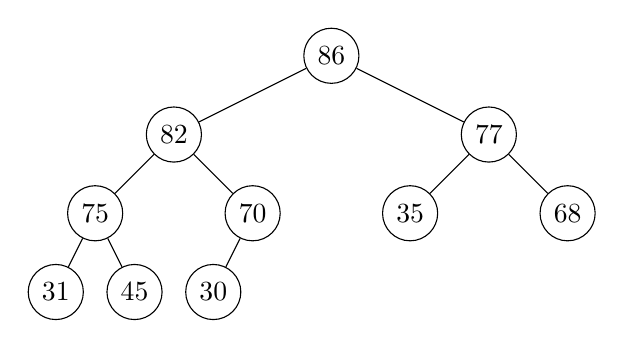
\begin{tikzpicture}[v/.style={circle,draw,inner sep=1pt,minimum size=7mm},
  level distance=10mm, level 1/.style={sibling distance=40mm},
  level 2/.style={sibling distance=20mm}, level 3/.style={sibling distance=10mm}]
\node[v] {86}
  child {node[v] {82}
    child {node[v] {75} child {node[v] {31}} child {node[v] {45}}}
    child {node[v] {70} child {node[v] {30}} child[missing] {}}}
  child {node[v] {77}
    child {node[v] {35}}
    child {node[v] {68}}};
\end{tikzpicture}
\end{center}

\begin{itemize}
\item 插入 25：放在索引 11，父節點是索引 $\lfloor 11/2 \rfloor = 5$ 的 70。 $25 < 70$，不動。
\item 插入 16：放在索引 12，父節點是索引 6 的 35。 $16 < 35$，不動。
\item 插入 12：放在索引 13，父節點是索引 6 的 35。 $12 < 35$，不動。
\end{itemize}

結果：
\begin{center}
\begin{tabular}{l*{13}{c}}
\toprule
索引 & 1 & 2 & 3 & 4 & 5 & 6 & 7 & 8 & 9 & 10 & 11 & 12 & 13 \\
\midrule
鍵 & 86 & 82 & 77 & 75 & 70 & 35 & 68 & 31 & 45 & 30 & \textbf{25} & \textbf{16} & \textbf{12} \\
\bottomrule
\end{tabular}
\end{center}
25 成為 70 的右子節點，16、12 成為 35 的左、右子節點。 這題的陷阱在於以為一定要交換：插入只在
新鍵比父節點大時才往上移，這三個鍵都比父節點小，所以每次只比較一次就結束。
\end{pastsoln}
